%\newpage
\section{Measurement of Semiconductors}
One probe pin is assumed to be the negative side of the component.
Another pin is assumed to be the positive side of the component.
For a first test, the components positive side is directly connected to VCC.
The negative side is connected with the \(680\Omega\) resistor to GND.
The test probe (third pin, also called TriStatePin) is first connected with the \(680\Omega\) resistor
for 10 ms to GND. The voltage of the negative probe pin is read, during  the TriStatePin is
switched to Input (High Impedance). It is assumed that the tested part can be
a N-Channel MOSFET and the gate should be discharged.
If the readed voltage is above 976mV, the next test assume, that the tested part can
also be a P-Channel MOSFET and for this a 10ms switch of the TriStatePin with the \(680\Omega\) resistor
to the VCC side is done.
Also for this case the voltage at the negative Probe pin is read with a currentless TriStatePin.
If the voltage of the negative pin is greater than 455mV, additional tests are made to differ
N-Channel JFET or D-MOSFET (depletion) and P-Channel JFET or P-MOSFET. 
The MOSFET versions can be differed by the missing of gate current in any state
of the TriStatePin.

To get parameters of the depletion types, they will be measured with a \(680 \Omega\) resistor at
the source pin, as shown in figure \ref{fig:JFETcd} . This measurement will be done instead of the
usually measurement of current with the gate hold at source level, because
the \(I_\mathrm{DSS}\) current of the FET transistor can often not be reached
with the relative high resistance of the \(680 \Omega\) resistor.

\begin{figure}[H]
\centering

\includegraphics[]{../FIG/JFETcd.eps}
\caption{Measurement of the  Gate-Source voltage and Source current of a N-JFET transistor}
\label{fig:JFETcd}
\end{figure}

If the component has no current between positive probe and negative probe without signal at the
TristatePin, the next tests are specified in the next section \ref{sec:pnp}.
If current was detected, the next test is described in the diode section \ref{sec:diode}.

\subsection{Measurement of PNP Transistor or P-Channel-MOSFET}
\label{sec:pnp}
First the current amplification factor is measured with common collector for the assumed PNP transistor.
The measuring situation is shown in figure \ref{fig:pnpcc}.
If the measured voltage at the Base (\(UB\)) is above 9mV with the \(680\Omega\) resistor,
the hFE is build as \(hFE = \frac{UE-UB}{UB}\). The voltage \(UE\) is the difference of the Emitter-voltage to VCC.
The difference between the \(22\Omega\) and \(19\Omega\) resistors are not respected.
If the \(UB\) voltage is below 10mV, the measurement is done with the \(470k\Omega\) resistor at the base.
In this case the current amplification factor is build as \(hFE = \frac{UE \cdot 470000}{UB \cdot (680+22)}\).

\begin{figure}[H]
\centering

\includegraphics[]{../FIG/PNPcc.eps}
\caption{hFE measurement of PNP transistor with common collector circuit }
\label{fig:pnpcc}
\end{figure}

Next the tests with common emitter are done for the assumed PNP transistor.
The positive side of component is now direct connected to VCC, the negative side \(680\Omega\) resistor
is connected to GND as shown in Figure \ref{fig:pnpce}. 
If the negative side of component has a voltage of above 3.4V, when the base side \(680\Omega\) resistor 
was connected to GND, it must be a PNP transistor or a P-Channel FET. This can be easy find out by
analysing the base voltage. If the base voltage is greater 0.97V, it must be a PNP.
For measuring the current amplification factor, the \(470k\Omega\) resistor is taken as Base resistor
instead of the \(680\Omega\).
The current amplification factor is build by \(hFE = \frac{(UC-UC0) \cdot 470000}{UB \cdot (680+19)}\) .
The voltage UC0 is the voltage at the colletor resistor without base current.
The higher current amplification factor is assumed to be the right one, this one or the one found with
the common collector circuit.

The values found for the PNP are only valid, if a second
set of measurements is done. In order to prevent detecting the PNP in the inverse mode
(collector and emitter are swapped), the measurement with the higher current amplification is taken as
the right one.
If base voltage is lower than 0.97V, it must be a P-E-MOS. In this case the gate threshold voltage is measured
by switching the gate slowly with the \(470k\Omega\) resistor up and down, waiting for a digital
input signal change of the Drain side and then read the voltage of the gate pin.
\begin{figure}[H]
\centering

\includegraphics[]{../FIG/PNPce.eps}
\caption{test and hFE measurement of PNP transistor with common emitter circuit }
\label{fig:pnpce}
\end{figure}

\subsection{Measurement of NPN Transistor or N-Channel-MOSFET}
The measuring of NPN-Transistors begin in the same way as PNP-Transistors with measuring
the current amplification factor in the common collector circuit.
First measurement is done with a \(680\Omega\) base resistor switched to VCC. If the
voltage at the base resistor ist too low, the \(470k\Omega\) resistor is taken instead.
Measurement then continues with the common emitter circuit as shown in figure \ref{fig:npnce}.
\begin{figure}[H]
\centering

\includegraphics[]{../FIG/NPNce.eps}
\caption{test and hFE measurement of NPN transistor with common emitter circuit }
\label{fig:npnce}
\end{figure}
If the voltage of collector sinks below 1.6V, when the \(680\Omega\) base resistor is connected to VCC,
ist must be a NPN, N-Channel MOSFET or Thyristor/Triac.
With two simple tests a Thyristor or Triac can be identified. If the gate pin resistor is connected
for 10ms to GND and than made currentless, the current at the anode should stay.
If then the anode resistor is short connected to GND and reconnected to VCC, the Thyristor should not
trigger again (no current). Please keep in mind, that only low power Thyristors can be tested, because
the holding current of the tester can reach only 6mA. If both tests attest a Thyristor, further tests with
reverse polarity are done to exclude or confirm a Triac.

If neither Thyristor nor Triac could be confirmed, it can be a NPN or N-Channel E-MOSFET.
The Base voltage of a NPN Transistor will be near the Emitter voltage, so this type can be identified definitely.
The current amplification factor in the common emitter circuit is build by \(hFE = \frac{(VCC-UC-UC0)\cdot 470000}{(VCC-UB)\cdot (680+22)}\).
If the voltage of the Base or better Gate  shows, that there is no or little current, part will be a N-Channel E-MOS 
(Enhancement MOSFET). In this case the threshold voltage is measured by switching the Gate slowly with
the \(470k\Omega\) resistor to VCC and GND, waiting for a digital input signal change of the Drain side and
then read the voltage of the Gate pin. This measurement is done eleven times with ADC results accumulated as
shown in Figure~\ref{fig:eleven}. The result is multiplied by four and divided by 9 to get the voltage in mV resolution.
\begin{figure}[H]
\centering
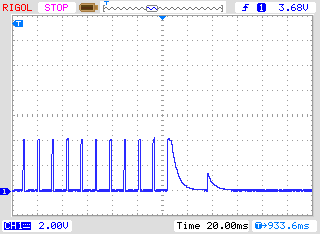
\includegraphics[]{../PNG/IRFU120gate.png}
\caption{measuring of threshold voltage of N-Channel-MOSFET}
\label{fig:eleven}
\end{figure}

\subsection{Measurement of Diodes}
\label{sec:diode}
If current is detected with the pre-tests, the behavior of the part will be checked to
be a diode. The flow voltage with the \(680\Omega\) resistor must be between 0.15V and 4.64V.
The flux voltage with the \(680\Omega\) must be greater than 1.125 times the flux voltage with
the \(470k\Omega\) resistor and sixteen times the flux voltage with the \(470k\Omega\) must be
greater than the flux voltage with the \(680\Omega\) resistor.
Additionally the afterward renewed measurement with the \(470k\Omega\) resistor should not have a higher voltage than
the previous measurement with the \(680\Omega\) resistor.
I hope, that this behavior identifies always a diode. The identification of a diode by no current flow
in the opposite direction is not possible with a inverse parallel diode.
If only a single diode is detected, the residual current in reverse direction is measured with
the \(470k\Omega\) resistor at 5V. The resolution is about \(2nA\).
If the residual current is greater as \(5.3\mu A\) (voltage at
the \(470k\Omega\) is more than 2.5V), the measurement is done with the \(680\Omega\) instead.
Then the resolution is only about \(1\mu A\).
Furthermore  the capacity in reverse direction is also measured for single diodes.



\subsection{Results of different measurements}
The following three tables shows results of different test probes 
with one ATmega8 processor and two different software versions of a ATmega168 processor.
The measurement of the inverse capacity value for the double diode MBR4045PT is 
only possible with cooling. This will be caused by high residual current of this 40A diode.
Also the capacity value of the inverse base emitter diode of the germanium transistor AC128 can
only be measured with cooling.

\begin{table}[H]
  \begin{center}
    \begin{tabular}{| l | c | c | c |}
    \hline
           & Mega8@8MHz & Mega168 @8MHz & Mega328 @8MHz \\
 Diode Type  &                  &                  &                  \\
    \hline
    \hline
1N4148     & Diode, 715mV,        & Diode, 718mV,            & Diode, 715mV,           \\
           &               1pF    &               0pF, 2nA   &               1pF, 4nA  \\
    \hline
1N4150     & Diode, 665mV,        & Diode, 672mV,            & Diode, 666V,           \\
           &               1pF    &               1pF, 4nA   &              2pF, 6nA  \\
    \hline
BA157      & Diode, 619mV,        & Diode, 621V,              & Diode, 615mV,            \\
           &               19pF   &              17pF, 12nA   &               18pF, 12nA \\
    \hline
BY398      & Diode, 538mV,        & Diode, 541mV,             & Diode, 537mV,            \\
           &               16pF   &               14pF, 63nA  &               15pF, 63nA \\
    \hline
1N4007     & Diode, 650mV,        & Diode, 655mV,            & Diode, 650mV,           \\
           &               13pF   &               10pF, 6nA  &               13pF, 6nA \\
    \hline
LED green  & Diode, 1.96V, 5pF    & Diode, 1.95V, 4pF   & Diode, 1.95V, 4pF \\
    \hline
ZPD2,7     & 2xDi, 743mV, 2.53V   & 2xDi, 737mV, 2.52V  & 2xDi, 733mV, 2.51V \\
    \hline
BU508A B+E & Diode, 609mV,        & Diode, 611mV,                & Diode, 606mV,              \\
           &               5.15nF &               5.20nF, 0.39uA &               5.25nF, 0.4uA\\
    \hline
BU508A B+C & Diode, 582mV,        & Diode, 586mV,             & Diode, 587mV,            \\
           &               256pF  &               255pF, 21nA &               259pF, 19nA\\
    \hline
AC128 B+E  & Diode, 272mV,        & Diode, 277mV,              & Diode, 273mV,             \\
           &               0pF    &               0pF, 2.2uA   &               0pF, 2.3uA  \\
    \hline
AC128 B+E  &                      &                     & Diode, 349mV,               \\
cooled     &                      &                     &               140pF, 0.57uA \\
    \hline
MBR20100CT & 2xDi, 337mV, 337mV   & 2xDi, 338mV, 338mV  & 2xDi, 336mV, 335mV  \\
    \hline
MBR20100CT & Diode, 337mV,        & Diode, 339mV,             & Diode, 337mV,            \\
           &               345pF  &               351pF, 29nA &               350pF, 25nA\\
    \hline
MBR4045PT  & Diode, 243mV,        & Diode, 233mV,               & Diode, 235mV,              \\
cooled     &               1.80nF &               1.94nF, 1.7uA &               1.95nF, 1.8uA\\
    \hline
SF38G      & Diode, 519mV,        & Diode, 521mV,            & Diode, 516mV,            \\
           &               107pF  &               105pF, 2nA &               106pF, 2nA \\
    \hline
    \end{tabular}
  \end{center}
  \caption{measurement results of diode testing}
  \label{tab:diodes} 
\end{table}

\begin{table}[H]
  \begin{center}
    \begin{tabular}{| l | c | c | c |}
    \hline
     Transistor & Mega8@8MHz & Mega168 @8MHz & Mega328 @8MHz \\
     Type   &                  &                  &                  \\
    \hline
    \hline
BU508A      & NPN, B=9, 602mV     & NPN, B=10, 594mV    & NPN, B=9, 591mV   \\
    \hline
2N3055      & NPN, B=20, 553mV    & NPN, B=22, 545mV    & NPN, B=21, 542mV  \\
    \hline
BC639       & NPN, B=180, 628mV   & NPN, B=215, 623mV   & NPN, B=173, 620mV \\
    \hline
BC640       & PNP, B=216, 635mV   & PNP, B=178, 635mV   & PNP, B=183, 600mV \\
    \hline
BC517       & NPN, B=26.1k, 1.20V & NPN, B=27.8k, 1.21V & NPN, B=26.1k, 1.20V\\
    \hline
BC516       & PNP, B=77.6k, 1.20V & PNP, B=81.1k, 1.19V & PNP, B=81.7k, 1.18V\\
    \hline
BC546B      & NPN, B=381, 659mV   & NPN, B=380, 653mV   & NPN, B=430, 675mV \\
    \hline
BC556B      & PNP, B=285, 689mV   & PNP, B=250, 688mV   & PNP, B=262, 654mV \\
    \hline
AC128 (Ge.) & PNP, B=63, 190mV    & PNP, B=61, 184mV    & PNP, B=59, 182mV  \\
    \hline
BRY55/200   & Thyristor           & Thyristor           & Thyristor        \\
    \hline
MAC97A6     & Triac               & Triac               & Triac        \\
    \hline
    \end{tabular}
  \end{center}
  \caption{measurement results of bipolar transistor testing}
  \label{tab:bipolar} 
\end{table}

Some results are different to the earlier results of the software of Markus Frejek.
For example a darlington transistor BC517 has been measured by the older software
with a hFE of 797 .
and a base emitter voltage of 1438mV.
This will be caused by the additional measurement of current amplification with common collector circuit.
The base emitter voltage is measured by the older Version as separate diode test with 1438mV.
Now the base emitter voltage is measured with the state of current amplification testing (1.20V).

The following table shows the measurement results for germanium transistors, which are extra problematic
to measure because of the temperatur dependent and high residual collector current.
The results of the original version of Markus F. and the results of the actual 1.08k version are
compared together. The 1.08k version for a ATmega328 measures the current amplification factor with
common collector and common emitter circuit, the higher result will be shown.
The 1.08k version for the ATmega168 measures only with common collector circuit.

\begin{table}[H]
  \begin{center}
    \begin{tabular}{| l | c | c | c |}
    \hline
 Transistor & Mega8@1MHz          & Mega168 @8MHz       & Mega328 @8MHz    \\
    Type    & Original Version    & Version 1.08k       & Version 1.08k  \\
            & Markus F.           &                     &        \\
    \hline
    \hline
AC128       & PNP, B=52, 279mV    & PNP, B=61, 185mV    & PNP, B=60, 190mV    \\
    \hline
AC116-65    & PNP, B=505, 378mV   & PNP, B=56, 237mV    & PNP, B=76, 144mV    \\
    \hline
AC116-145   & PNP, B=485, 294mV   & PNP, B=83, 212mV    & PNP, B=167, 156mV   \\
    \hline
AC176-65    & NPN, B=98, 235mV    & NPN, B=52, 146mV    & NPN, B=57, 97mV     \\
    \hline
GC122       & PNP, B=84, 368mV    & PNP, B=56, 186mV    & PNP, B=58, 117mV    \\
    \hline
GC301       & PNP, B=48, 289mV    & PNP, B=40, 183mV    & PNP, B=40, 189mV    \\
    \hline
    \end{tabular}
  \end{center}
  \caption{Measurement results of bipolar junction germanium transistors}
  \label{tab:germanium}
\end{table}




\begin{table}[H]
  \begin{center}
    \begin{tabular}{| l | c | c | c |}
    \hline
    \hline
             & Mega8@8MHz       & Mega168 @8MHz    & Mega328 @8MHz \\
 FET Type     &                  &                  &               \\
    \hline
    \hline
ZVNL120A     & N-E-MOS,D, 1.6V  & N-E-MOS,D, 1.5V  & N-E-MOS,D, 1.5V \\
             & 147pF            & 139pF            & 140pF \\
    \hline
IRF530N      & N-E-MOS,D, 3.6V  & N-E-MOS,D, 3.6V  & N-E-MOS,D, 3.6V \\
             & 1.55nF           & 1.54nF           & 1.56nF \\
    \hline
BS170        & N-E-MOS,D, 2.6V  & N-E-MOS,D, 2.6V  & N-E-MOS,D, 2.6V \\
             &  78pF            &  68pF            &  70pF \\
    \hline
IRL3803      & N-E-MOS,D, 2.3V  & N-E-MOS,D, 2.3V  & N-E-MOS,D, 2.3V \\
             & 9.81nF           & 9.71nF           & 9.80nF \\
    \hline
IRFU120N     & N-E-MOS,D, 4.2V  & N-E-MOS,D, 4.2V  & N-E-MOS,D, 4.2V \\
             & 909pF            & 913pF            & 920pF \\
    \hline
BUZ71A       & N-E-MOS,D, 3.2V  & N-E-MOS,D, 3.2V  & N-E-MOS,D, 3.2V \\
             & 714pF            & 708pF            & 714pF \\
    \hline
ZVP2106A     & P-E-MOS,D, 3.2V  & P-E-MOS,D, 3.2V  & P-E-MOS,D, 3.2V \\
             & 122pF            & 115pF            & 117pF \\
    \hline
IRF5305      & P-E-MOS,D, 3.6V  & P-E-MOS,D, 3.6V  & P-E-MOS,D, 3.6V \\
             & 2.22nF           & 2.22nF           & 2.24nF \\
    \hline
BS250        & P-E-MOS,D, 2.6V  & P-E-MOS,D, 2.6V  & P-E-MOS,D, 2.6V \\
             & 53pF             & 43pF             & 44pF \\
    \hline
IRFU9024     & P-E-MOS,D, 3.5V  & P-E-MOS,D, 3.6V  & P-E-MOS,D, 3.5V \\
             & 937pF            & 945pF            & 952pF \\
    \hline
J310         & N-JFET           & N-JFET           & N-JFET\\
Idss=24-60mA & I=3.1mA Vgs=2.2V & I=3.1mA Vgs=2.2V & I=3.1mA Vgs=2.2V \\
    \hline
2N5459       & N-JFET           & N-JFET           & N-JFET\\
Idss=4-16mA & I=2.1mA Vgs=1.5V & I=2.1mA Vgs=1.5V & I=2.1mA Vgs=1.5V \\
    \hline
BF256C       & N-JFET           & N-JFET           & N-JFET\\
Idss=11-18mA & I=3.4mA Vgs=2.4V & I=3.4mA Vgs=2.4V & I=3.4mA Vgs=2.4V \\
    \hline
BF245A       & N-JFET           & N-JFET           & N-JFET\\
Idss=2-6mA   & I=1.1mA Vgs=.75V & I=1.1mA Vgs=0.75V & I=1.1mA Vgs=0.75V \\
    \hline
BF245B       & N-JFET           & N-JFET           & N-JFET\\
Idss=6-15mA  & I=2.5mA Vgs=1.7V & I=2.5mA Vgs=1.7V & I=2.5mA Vgs=1.7V \\
    \hline
BF245C       & N-JFET           & N-JFET           & N-JFET\\
Idss=12-25mA & I=3.9mA Vgs=2.7V & I=3.9mA Vgs=2.7V & I=3.9mA Vgs=2.7V \\
    \hline
J175        & P-JFET           & P-JFET           & P-JFET\\
Idss=7-60mA & I=3.2mA Vgs=2.2V & I=3.2mA Vgs=2.2V & I=3.2mA Vgs=2.2V \\
    \hline
2N5460      & P-JFET           & P-JFET           & P-JFET\\
Idss=1-5mA  & I=0.78mA Vgs=0.54V & I=0.77mA Vgs=0.54V & I=0.78mA Vgs=0.54V \\
    \hline
    \end{tabular}
  \end{center}
  \caption{measurement results of MOS transistor testing}
  \label{tab:mos} 
\end{table}
